\Chapter{PROSPECT Experiment}
    
    The RAA described in Chapter~\ref{Ch2} leads to the need for experiments capable of probing short baseline sterile neutrino oscillation, as well as directly measuring the flux and spectrum of a  reactor with a high concentration of a single fission isotope. 
    The experiment has to meet the requirements of :
    \begin{itemize}
        \item Sub-10~m baseline from a reactor with a compact reactor size. 
        \item Fission reactor whose neutrino production is from a single isotope.
        \item Good IBD position reconstruction resolution for oscillation measurement.
        \item High energy resolution to precisely measure neutrino spectrum.
    \end{itemize}
    
    PROSPECT~\cite{bib:prospect_physics, bib:prospect_nim}, the Precision Reactor Oscillation and SPECTrum experiment, was designed and built to directly measure the neutrino flux and spectrum from the HFIR located at ORNL~\cite{bib:hfir}. 
    PROSPECT's antineutrino detector (AD) covers baselines from 7~m to 9~m with a segmented LS volume.
    The goals of PROSPECT are to probe eV-scale sterile neutrino oscillation by the observation of \nuebar disappearance, and to precisely measure the  reactor neutrino spectrum from $^{235}$U.
    
\Section{HFIR Reactor}

    HFIR is a high enrichment $^{235}$U (HEU) research fission reactor whose $^{235}$U enrichment is 93\% on average.
    The key parameters of the HFIR core relevant to PROSPECT neutrino measurements are listed in Table~\ref{tab:HFIR}.
\begin{table}[h]
    \centering
    \caption[The properties of HFIR]{The properties of HFIR.}
    \begin{tabular}{cc}
    \hline
    \hline
    Parameter  & Value   \\
    \hline
    Power    & 85~MW \\
    Dimensions     & 435~mm (diameter) $\times$ 508~mm (height) \\
    $^{235}$U enrichment & 93\% \\
    Neutrino source & $\sim$99\% from $^{235}$U \\
    Reactor cycle & $\sim$25~day on, $\sim$30~day off \\
    \hline
    \end{tabular}

\label{tab:HFIR}
\end{table}

\begin{figure}[h!]
    \centering
    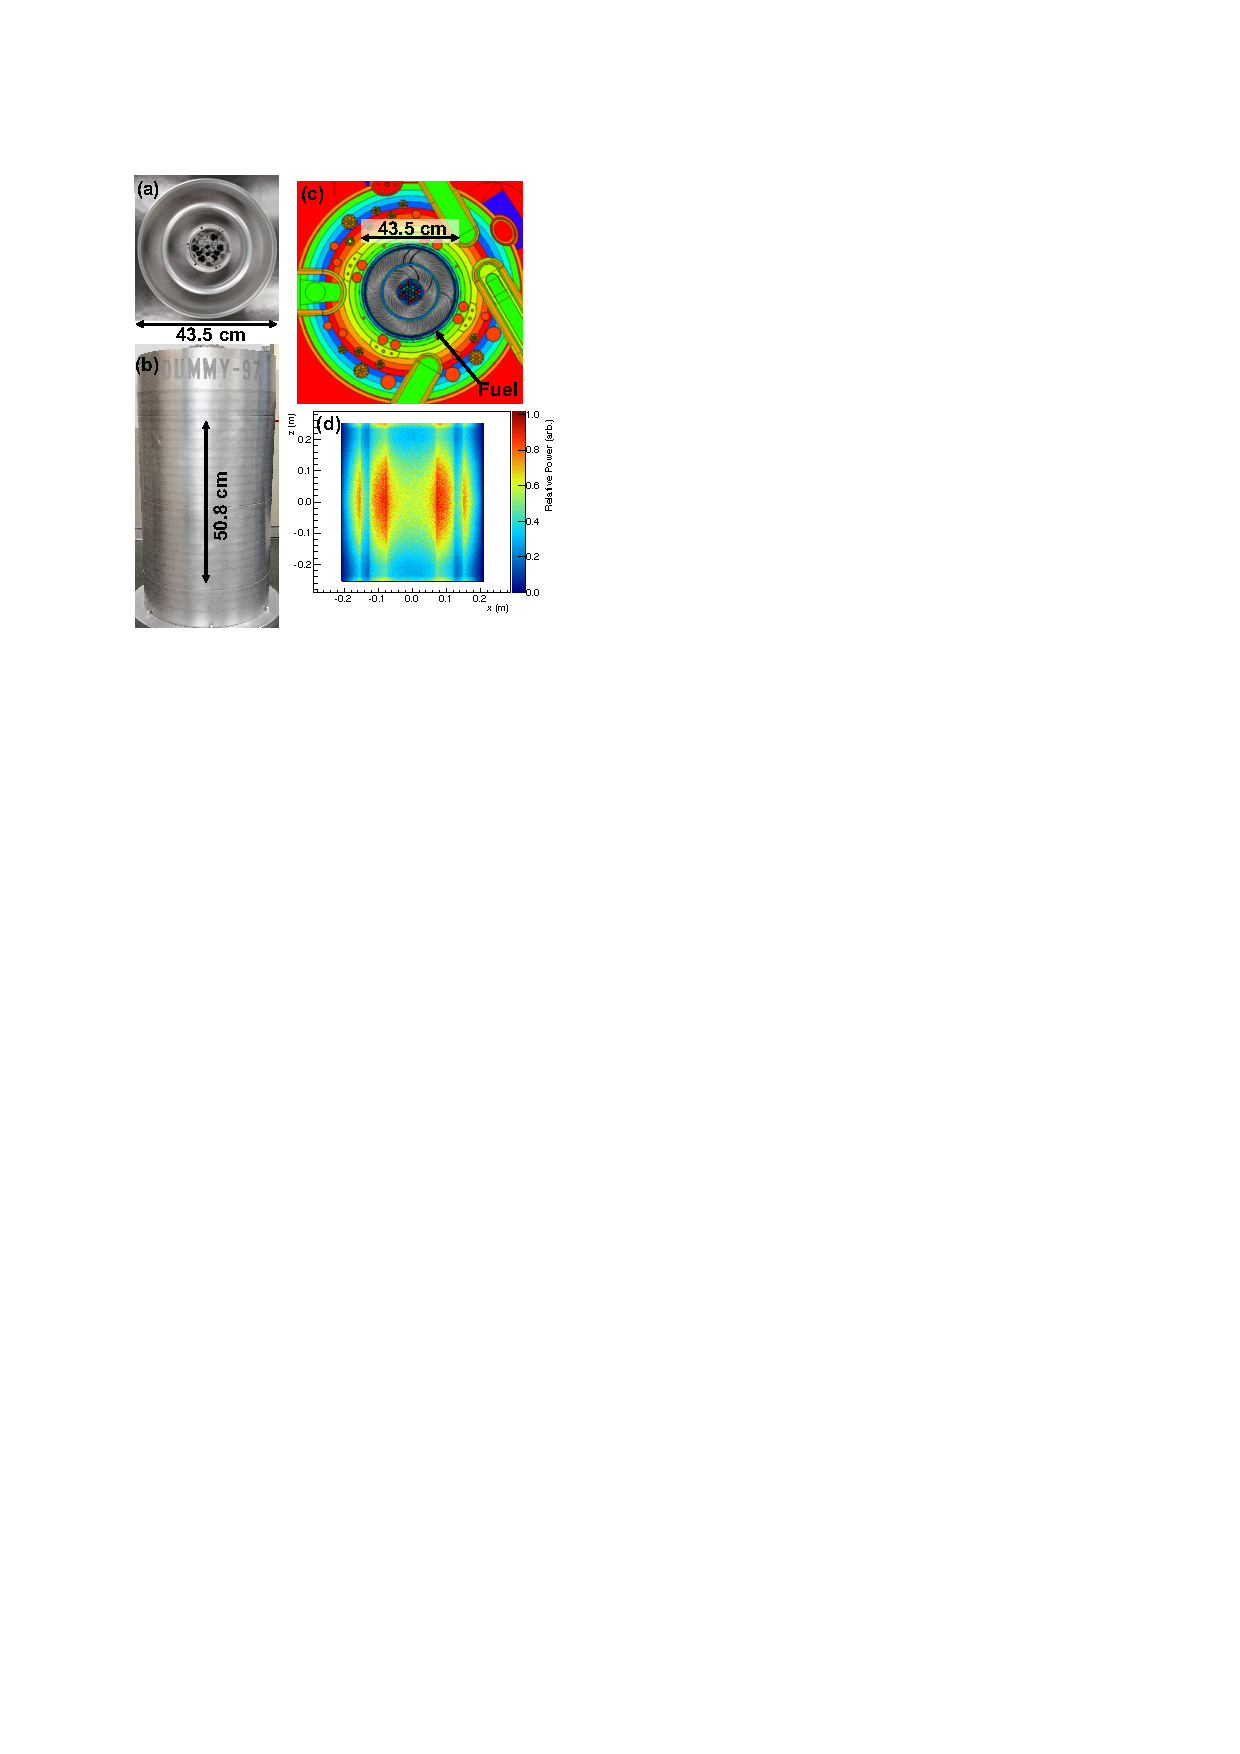
\includegraphics[width=0.5\textwidth]{Figures/HFIR.pdf}
    \caption[The dimensions and power distribution of HFIR]{A model of the reactor~\cite{bib:prospect_nim} parameters.
     (a) and (b) are the diameter and height of the HFIR core.
    The location of the HFIR core in a detailed reactor system simulation is indicated in (c).
    (d) is a projection of the fission power density of HFIR at the x-z plane.}
    \label{fig:HFIR}
\end{figure}

    HFIR is a cylindrical fission reactor.
    Its compact size, as shown in Table~\ref{tab:HFIR} and Figure~\ref{fig:HFIR}, is ideal for constraining the uncertainty in neutrino baselines.
    To maintain its high $^{235}$U enrichment, the HFIR reactor is operated in relatively short reactor cycles.
    In this case, the fuel evolution of fissile isotopes is negligible.
    
    The HFIR facility also brings unique background challenges for neutrino measurements. 
    Due to availability of an experiment site at very short baseline, the PROSPECT AD is exposed to cosmic ray backgrounds with minimal overburden. 
    The detector also faces reactor correlated background, e.g., the background neutrons generated from the reactor, and the gamma-ray background from neutron capture on materials in the piping of the facility.
    A comprehensive background characterization was therefore organized in the research and development (R\&D) phase of PROSPECT~\cite{bib:prospect_background}. 
    Figure~\ref{fig:prospect_background} shows the amplitude of the gamma and neutron background.
    The detector and additional background shielding were designed based on this background survey.
    
\begin{figure}
    \centering
    %\vspace{0pt}
    \includegraphics[width=0.47\textwidth, valign=t]{Figures/NeutronBGMap.pdf}
    %\vspace{0pt} 
    \includegraphics[width=0.51\textwidth, valign=t]{Figures/GammaBGMap.pdf}
    \caption[Local background distribution at the HFIR facility]{(Left) The reactor correlated neutron background rate (nSv/h) shown in a map of the HFIR site where PROSPECT is deployed.
    (Right) The local $\gamma$ ray background rate (Hz) shown in the same map.
    }
    \label{fig:prospect_background}
\end{figure}

\Section{Detector Design}

    The PROSPECT AD is a $\sim$4~ton $^{6}$Li-doped LS ($^{6}$LiLS) detector deployed at 7-9~m baselines from the HFIR core.
    The critical parameters of the PROSPECT AD are shown in Table~\ref{tab:PROSPECT_AD}.
    The schematic of detector deployment at the HFIR facility is shown in Figure~\ref{fig:PROSPECT_LAYOUT}.
\begin{table}[h]
    \centering
    \caption[Key parameters of the PROSPECT AD]{The key parameters of the PROSPECT AD~\cite{bib:prospect_nim}.}
    \begin{tabular}{cc}
    \hline
    \hline
    Parameter  & Value   \\ 
    \hline
    Target volume \& mass    & 3760 liters, 3.68 tons\\
    Target dimension & 1.176\,m wide $\times$ 2.045\,m long  $\times$ 1.607\,m tall \\
    Baseline     & 7.9~m \\
    Liquid scintillator & EJ-309 based LS with $<$0.1\% $^{6}$Li \\
    LS energy resolution & 4.5\% \\
    Segments & 14 horizontal $times$ 11 vertical \\
    Segment dimension & 1.176\,m wide $\times$ 14.5~cm long  $\times$ 14.5~cm tall \\
    Light collection & diameter = 12.7~cm (5~inch) PMTs\\
    Position resolution & $\sigma_X$ = 14.5~cm,  $\sigma_Y$ = 14.5~cm,  $\sigma_Z \approx$ 5~cm \\
    \hline
    \end{tabular}
    \label{tab:PROSPECT_AD}
\end{table}
\begin{figure}
    \centering
    %\vspace{0pt}
    \includegraphics[width=0.6\textwidth]{Figures/Layout.pdf}
    \caption[The layout of the PROSPECT experiment]{The layout of the PROSPECT experiment.
    The PROSPECT AD is deployed 7.9~m from the reactor center to the detector center.
    An additional on-site lead shield was installed between the reactor pool and the AD to eliminate local gamma-ray backgrounds.
    }
    \label{fig:PROSPECT_LAYOUT}
\end{figure}
    
    The anatomy of the PROSPECT AD is shown in Figure~\ref{fig:PROSPECT_AD}.
    The inner volume of the detector is contained in a liquid-tight acrylic tank filled with the $^{6}$LiLS, which is made from EJ-309 base, an organic LS \cite{bib:lspaper}.
    The acrylic tank is shielded by layers of water, polyethylene, lead, and borated polyethylene, respectively from the outside to inside to suppress neutron and gamma backgrounds.
    The designed energy resolution is 4.5\% to optimize PROSPECT's IBD spectrum measurement.
    An advantage of utilizing EJ-309 is its pulse shape discrimination (PSD) capability which makes the PROSPECT AD sensitive to particle identity, which is described in detail in Section~\ref{sec:detection}.
    The purified $^{6}$Li is loaded as a main neutron capture isotope through dissolved LiCl in the scintillator.
    A small amount of $^{227}$Ac was also uniformly spiked in the LS for active calibration of segment volume differences.

\begin{figure}
    \centering
    %\vspace{0pt}
    \includegraphics[trim = 0cm 2cm 0cm 2cm, clip,width=0.8\textwidth]{Figures/DetectorDesign.pdf}
    \caption[The design of the PROSPECT AD]{The design of the PROSPECT AD, consisting an inner volume and surrounding layers of shielding.
    The inner detector includes $^{6}$LiLS, the optical grid, PMTs, and the calibration system.
    }
    \label{fig:PROSPECT_AD}
\end{figure}

    The inner volume of the PROSPECT AD is optically segmented by a light-weight optical grid subsystem~\cite{bib:prospect_og}.
    The optical grid consists of highly reflective carbon fiber backed separators dividing the LS volume into 14$\times$11 identical longitudinal segments. 
    Each segment is enclosed by two 12.7~cm diameter PMTs at its two ends.
    Schematics of the PROSPECT AD inner volume are shown in Figure~\ref{fig:active_volume}.
    The segment with the largest LS light signal is identified as the interaction point (x- and y-direction) of an incident particle.
    The readout of PMTs, which are housed in mineral-oil filled acrylic modules (PMT optical modules) on both sides of each segment, allows for timing- and charge-based position reconstruction along the axis (z-direction) of each segment~\cite{bib:P50, bib:P20}.
    Hence, the optical grid makes the PROSPECT AD able to reconstruct incident particles' 3D positions, which is an essential function for cosmic ray rejection and oscillation measurements.
    
\begin{figure}[h]
    \centering
    %\vspace{0pt}
    \includegraphics[width=0.7\textwidth]{Figures/PROSPECTAD_active.pdf}
    \caption[The inner volume of the PROSPECT AD]{Schematic of the inner volume of the PROSPECT AD.
    (Top) A side view to the X,Y plane of the AD, the red grids represent segments assembled with ElectronTubes PMTs and the light blue grids represent segments with Hamamatsu PMTs.
    (Bottom) A schematic of a single segment.
    }
    \label{fig:active_volume}
\end{figure}

\Section{Antineutrino Detection}
\label{sec:detection}

\Subsection{IBD signature}
	Similar to other reactor neutrino experiments, the PROSPECT AD detects \nuebar through the detection of the positron and neutron produced in the IBD process:
	\begin{equation}
        \nuebar + p \rightarrow n + e^+.
    \end{equation}	    
	The positron deposits its kinetic energy immediately in the LS by transferring the kinetic energy to molecular energy that generates scintillation light, a process described in detail in Chapter~\ref{Ch5}.
	Having lost most of its kinetic energy, positron-electron annihilation produces two 511~keV gammas moving in opposite directions. 
	The IBD neutron produced, with keV-scale kinetic energy, is decelerated within 50~\textmu s and then captured by a nucleus in the LS. 
	The main neutron capturing isotope in the PROSPECT AD is $^6$Li, with approximately 80\% of the total neutron capture fraction.
	The $n$-Li capture process,
	\begin{equation}
       	n+^6\textrm{Li} \rightarrow \alpha + ^3\textrm{H},
    \end{equation}
    brings an advantage for PROSPECT that the event signature includes only the recoil of $\alpha$ and $^3$H nuclei without energy loss. 
    The traveling distance of $\alpha$ and $^3$H produced are in the mm-scale.
    Thus, the $n$-Li capture event is restricted to a single segment.
    On the contrary, most of the historical reactor neutrino experiments utilizing Gd as the neutron capture solvent have to tag the neutron signal as a cascade of $\gamma$ rays with a total energy of approximately 8~MeV and a spreading light signal at the meter-scale.
 	The scintillation signal of the IBD produced positron, and its annihilation gammas are detected at the 10~ns scale after the IBD process, followed by the $\sim$50~\textmu s delayed neutron capture signal. 
 	Hence, the positron and neutron signals are referred to as prompt and delayed signals, respectively.
	A schematic of the IBD signals in PROSPECT is shown in Figure~\ref{fig:IBDscheme}.
\begin{figure}[h]
    \centering
    %\vspace{0pt}
    \includegraphics[width=0.7\textwidth]{Figures/IBDSchematic.pdf}
    \caption[IBD detection schematic]{A schematic of IBD detection in PROSPECT AD.
	An IBD event is tagged with time coincidence between the positron and the neutron events.
	The positron deposits its energy and annihilates in $\sim$10~ns after IBD process.
	Within $\sim$50~\textmu s after the IBD process, the neutron is mainly captured by $^6$Li, generating $\alpha$ and tritium with a total kinetic energy of 4.78~MeV (0.55~MeV electron equivalent).}
    \label{fig:IBDscheme}
\end{figure}

\Subsection{Prompt and Delayed Signal Discrimination}
	PROSPECT discriminates the prompt and delayed signal with PSD. 
	The pulse shape of scintillation light in EJ-309 contains short-lived and long-lived fluorescence components whose fractions in the light pulse are dependent on the $dE/dx$ of an ionizing particle. 
	Since the $dE/dx$ of charged nuclei is greater than the positrons and electrons, a significant difference of pulse shapes between the prompt and the delayed signals is shown as Figure~\ref{fig:PSD}.
	\begin{figure}[h]
    \centering
    %\vspace{0pt}
    \includegraphics[width=0.6\textwidth]{Figures/PSD.pdf}
    \caption[Pulse shape difference]{
	An example of the different pulse shape between a $\gamma$ ray-like signal and a neutron-like signal~\cite{bib:P50}.
	}
    \label{fig:PSD}
	\end{figure}
	For the ease of signal discrimination, a PSD parameter is defined as the tail fraction of the pulse integral, 
	\begin{equation}
       	\textrm{PSD} = \frac{Q_\textrm{tail}}{Q_\textrm{full}}.
    \end{equation}
    The time window of the tail integral, illustrated in Figure~\ref{fig:PSD}, is user defined to maximize the gamma-neutron discrimination~\cite{bib:P20}. 
    With event selection based on the reconstructed energy, timing and PSD value of a pulse, clear signal types can be distinguished as shown in Figure~\ref{fig:PSDvEvT}.
    	\begin{figure}[h]
    \centering
    %\vspace{0pt}
    \includegraphics[width=0.48\textwidth]{Figures/PSDvE.pdf}
    \includegraphics[width=0.48\textwidth]{Figures/PSDvT.pdf}
    \caption[Event selection based on PSD]{
    The IBD event selection based on PSD~\cite{bib:P50}.
    	(Left) The distribution of $^{252}$Cf neutron and gamma events in an energy and PSD parameter space.
    	A well-constrained distribution of $n$-Li capture can be seen at the low energy high PSD spot.
    	(Right) The distribution of prompt-delay pair event in the PSD and time coincidence parameter space, where the top-left spot is the distribution of IBD candidates.
	}
    \label{fig:PSDvEvT}
	\end{figure}
	
\Subsection{Energy and Position Reconstruction}
	The segmented nature of the PROSPECT AD allows particles with enough energy to travel through multiple segments.
	The energy of particles deposited in each segment is reconstructed by counting scintillation light collected by the PMTs on its ends.
	When both PMTs of a segment are triggered coincidentally, this light signal is referred to as a \textit{hit}.
	An event \textit{cluster} is defined as a group of hits in a 20~ns time interval. 
	The reconstructed energy of a particle is the sum of energy deposited in all segments of a cluster, as illustrated in Figure~\ref{fig:ClusterScheme}.
	The reconstructed event vertex $(x, y)$ position is defined as the location of the segment with the largest energy deposition in a cluster.
\begin{figure}[h]
    \centering
    %\vspace{0pt}
    \includegraphics[width=0.55\textwidth]{Figures/ClusterScheme.pdf}
    \caption[An illustration of an event cluster]{
	An illustration of an event cluster. The colored segments are segments which collected scintillation light within the cluster's time window.
	The reconstructed energy of this event is the summed energy detected by each segment hit in this cluster.
	The size and color of each colored box are correlated to the light collected in each PMT.
	The reconstructed positron is in the segment with the most significant light collection.
	}
    \label{fig:ClusterScheme}
\end{figure}
	
	An event vertex's $z$ position is reconstructed based on the charge and timing difference between the pair of PMTs' light signals.
	The schematic of a single segment's light collection is shown in Figure~\ref{fig:Zreconstruction}.
	Because of the light attenuation in the LS, the light collection by a PMT at one end decreases exponentially with increasing distance from that PMT to the vertex, resulting in the segment's total light collection non-uniformity along the $z$ direction.
	The detection timing difference between the PMTs is also dependent on the $z$ position, making it a useful tool in $z$ position reconstruction.
	Further discussion about the $z$ position calibration and reconstruction is detailed in Chapter~\ref{Ch6}.
	
\begin{figure}[h]
    \centering
    %\vspace{0pt}
    \includegraphics[width=0.6\textwidth]{Figures/Z_reconstruction.pdf}
    \caption[An illustration of a single segment light collection ]{
	An illustration of the light collection within one segment.
	When scintillation light is generated from an incident particle, the light is constrained in the segment by the specular reflective separators.
	The two PMTs on the ends of a segment detect different light and at a different time with respect to the vertex location.
	}
    \label{fig:Zreconstruction}
\end{figure}
	

